\documentclass[a4paper]{article}
\usepackage{tikz}
\usepackage{amsmath}
\usepackage[margin=2cm]{geometry}

\begin{document}

\begin{center}
    \textbf{Distancia punto a recta (manhattan con múltiples soluciones)}
\end{center}

\begin{center}
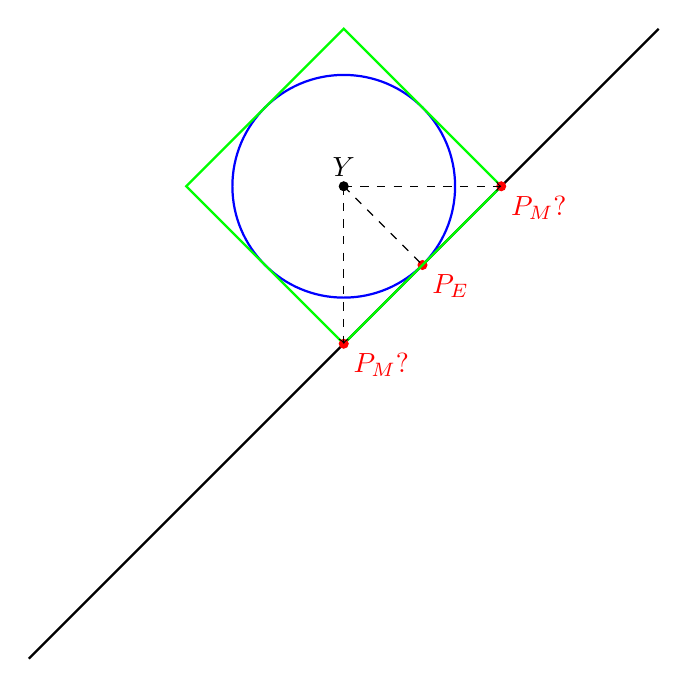
\begin{tikzpicture}[scale=2.0]
    % -----------------------------------------------------
    % 1) Recta (sin etiqueta)
    % -----------------------------------------------------
    \draw[thick] (-2,-2) -- (2,2);

    % -----------------------------------------------------
    % 2) Punto Y en (0,1)
    % -----------------------------------------------------
    \filldraw (0,1) circle (0.8pt) node[above] {$Y$};

    % -----------------------------------------------------
    % 3) Distancia Euclidiana: Círculo con centro en Y
    %    Proyección ortogonal en la recta: P_E = (0.5,0.5)
    % -----------------------------------------------------
    \draw[blue, thick] (0,1) circle ({1/sqrt(2)});
    \filldraw[red] (0.5,0.5) circle (0.8pt) node[below right] {$P_E$};
    \draw[dashed] (0,1) -- (0.5,0.5);

    % -----------------------------------------------------
    % 4) Distancia Manhattan: Rombo (L1)
    %    Vértices del rombo: (0,2), (1,1), (0,0), (-1,1)
    % -----------------------------------------------------
    \draw[green, thick] (0,2) -- (1,1) -- (0,0) -- (-1,1) -- cycle;

    % -----------------------------------------------------
    % 5) Dos puntos equidistantes sobre la recta tocando el rombo
    % -----------------------------------------------------
    \filldraw[red] (1,1) circle (0.8pt) node[below right] {$P_M?$};
    \filldraw[red] (0,0) circle (0.8pt) node[below right] {$P_M?$};

    % Flechas desde Y a los puntos sobre la recta
    \draw[->, dashed] (0,1) -- (1,1);
    \draw[->, dashed] (0,1) -- (0,0);

\end{tikzpicture}
\end{center}

\end{document}
